\chapter{Fundamentals}

\section{Differential Privacy}

Differential privacy is a concept for maintaining privacy when processing sensitive data that was introduced by \textcite{dwork:2006}. In principle, noise is added to query results in order to guarantee that the query result would occur with a similar probability for an \textit{adjacent data set}. The definition of what is considered an adjacent dataset depends on the application at hand, but it generally refers to datasets that differ in the contribution of data from one user. This guarantees that the influence of a single data point on the query result is limited. The similarity of the probabilities is determined by the \textit{privacy budget} $\epsilon$.

\begin{definition}
  \emph{\textbf{$\epsilon$-Differential Privacy}} A \textit{randomized mechanism} $\mathcal{M}: \mathcal{D} \rightarrow \mathcal{R}$ with domain $\mathcal{D}$ and range $\mathcal{R}$ satisfies $\epsilon$-differential privacy if for any two adjacent inputs $d$, $d' \in \mathcal{D}$ and for any subset of outputs $S \subseteq \mathcal{R}$ it holds that $$\Pr[\mathcal{M}(d) \in S] \leq e^{\epsilon} \Pr[\mathcal{M}(d') \in S]$$

\end{definition}

A less strict, but in practice much used definition also introduces a $\delta \in [0,1]$, which provides a probability that no privacy guarantees are observed. In \textcite{abadi:2016}, differential privacy is defined as follows:

\begin{definition}
  \emph{\textbf{$(\epsilon, \delta)$-Differential Privacy}} A \textit{randomized mechanism} $\mathcal{M}: \mathcal{D} \rightarrow \mathcal{R}$ with domain $\mathcal{D}$ and range $\mathcal{R}$ satisfies $(\epsilon, \delta)$-differential privacy if for any two adjacent inputs $d$, $d' \in \mathcal{D}$ and for any subset of outputs $S \subseteq \mathcal{R}$ it holds that $$\Pr[\mathcal{M}(d) \in S] \leq e^{\epsilon} \Pr[\mathcal{M}(d') \in S] + \delta$$
\end{definition}

Based on this definition, there are further theorems that enable the development of more complex DP algorithms. The first is the \textit{post-processing} theorem. It states that the further processing of data from a DP mechanism cannot further increase the loss of privacy. This property is important, for example, in order to be able to use models trained with privacy guarantees after training without hesitation. In addition, there are composition theorems that provide estimates for the fact that data is processed multiple times.

Noise is added using various mechanisms. Random values are drawn from distributions for which it has been proven that they fulfil the definition of differential privacy. For numerical queries, there is the Laplace mechanism, which draws the random values from the Laplace distribution, and the Gaussian mechanism, which draws the random values from the normal distribution. The Exponential Mechanism, for example, is suitable for categorical queries. Further details are described by \textcite{chang:2023}.

Since the strength of the added noise should be proportional to the greatest possible influence of a data point on the query result, it is also often necessary to limit the value range \parencite[p.31]{chang:2023}. For count queries, this influence is naturally limited to $1$, but if for example an average salary is requested, it is necessary to define the value range of the possible salaries. The greatest possible influence of a data point is called \textit{sensitivity}.

Machine learning models can also be regarded as queries on a data set. A DP mechanism can be applied to them at different points in time, as can be seen in \autoref{fig:design_principles_dpml}. Adding noise in the respective steps has various advantages and disadvantages.

\begin{figure}[tb]
  \centering
  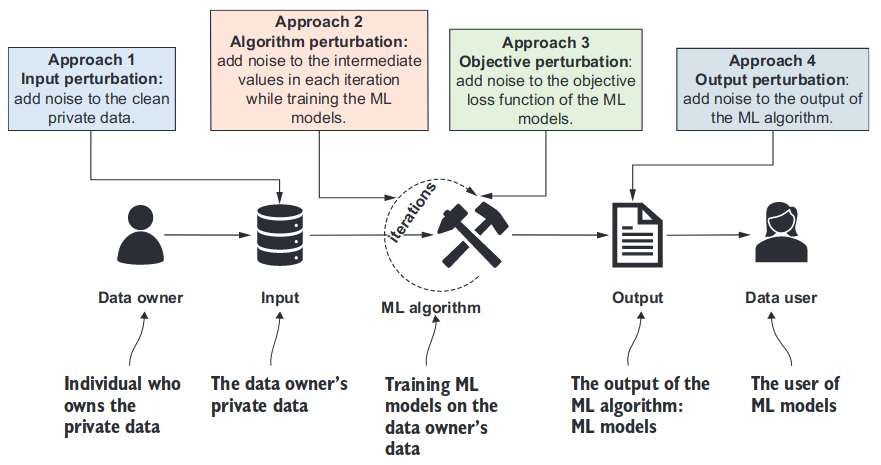
\includegraphics[width=0.7\textwidth]{Bilder/design_principles_dpml.png}
  \caption{Design principles of differentially private ML from \textcite{chang:2023}}
  \label{fig:design_principles_dpml}
\end{figure}

With \textit{input pertubation}, noise is added to the training data before training. This is easy to implement and versatile, but also requires a larger amount of noise as the data usually has a high \textit{sensitivity}.

Using \textit{algorithm pertubation}, the models are trained with unchanged data. In iterative algorithms, the intermediate results can be distorted in the individual steps. \textcite{abadi:2016}, for example, add noise to the gradients.

\textit{Output pertubation} adds noise to the outputs generated by the model. However, the method is not applicable if the model is to be published, as the number of requests to the model cannot be predicted and therefore no privacy guarantees are possible.

With \textit{Objective pertubation}, noise is added to the \textit{Objective function} for which the model is optimised.

The Differentially Private-Stochastic Gradient Descent (DP-SGD) presented by \textcite{abadi:2016} is now a widely used algorithm for training neural networks, on which many other works are based. It is based on the \textit{Stochastic Gradient Descent} (SGD), an iterative optimisation algorithm that is used in various machine learning methods. Compared to the SGD, the DP-SGD has some additional hyperparameters to fulfil the privacy guarantees:

\begin{itemize}
  \item \textbf{Noise scale $\sigma$} A factor by which the noise of the DP mechanism is controlled. 
  \item \textbf{Lot size $L$} The number of data points that are included in a gradient update.
  \item \textbf{Gradient norm bound $C$} All calculated gradients are clipped so that they have a maximum $\ell_2$ norm of $C$. This is necessary because noise with the Gaussian mechanism is added in the following and the sensitivity of vectors is defined via the $\ell_2$ norm. 
\end{itemize}

During training, these parameters affect how quickly a desired $(\epsilon, \delta)$ privacy budget is exhausted. In their results, \textcite{abadi:2016} show that the choice of these parameters (in addition to the parameters from the normal SGD) also has an effect on the accuracy of the model under a fixed privacy budget.

In addition to the specific algorithm, \textcite{abadi:2016} developed the \textit{Moments Accountant}, a method for estimating the loss of privacy during training, which is asympotically much more accurate than classical estimates using composition theorems. They prove this benefit in their work through empirical experiments.

In their paper, \textcite{mcmahan:2018} develop a variant of the \textit{Federated Averaging} (FedAvg) algorithm \parencite{mcmahan:2016} based on the work of \textcite{abadi:2016}, which ensures DP guarantees for users. Their goal is to train an LSTM model for \textit{Next-Word Prediction} on mobile devices. They transfer the definition of adjacent datasets to federated learning by defining the neighbourhood by adding or removing all data of a user. In their experiments, they show that the accuracy of the model can be maintained under DP guarantees, but at a higher computational cost.

The main changes compared to the non-private FedAvg are a limited sensitivity at the clients (by clipping) and at the server (by estimators of the aggregation with a limited range of values). In addition, the server adds noise to the aggregated update based on sensitivity.

\section{Federated Learning}

Federated Learning (FL) ist ein Optimierungsverfahren, bei dem einzelne Clients gemeinsam ein Modell trainieren, ohne dabei ihre eigenen Trainingsdaten mit anderen zu teilen. Dabei initialisiert ein Server ein Modell und seine Parameter. Danach wählt er eine Menge an Clients aus, mit denen in dieser Runde das Modell trainiert werden soll und schickt das Modell an diese. Die Clients optimieren das Modell auf ihren eigenen Daten und schicken das optimierte Update an den Server zurück. Dieser aggregiert alle Updates und aktualisiert damit sein Modell. Das ganze Verfahren wird über mehrere Runden wiederholt. 

Die lokale Optimierung und die Aggregation der Updates kann je nach Algorithmus variieren. FedAvg lässt die Clients mehrere Epochen auf ihren eigenen Daten trainieren und gewichtet die Updates bei der Aggregation nach der Menge der Daten, die die einzelnen Clients haben. FedSGD ist ein spezialfall von FedAvg, bei dem die Clients nur für einen Schritt trainieren und das Update dann zurückschicken \parencite{mcmahan:2016}. 

Das verteilte Training kann vor allem zwei Probleme mit sich bringen. Zunächst kann der Overhead für die Kommunikation sehr groß werden, gerade wenn über viele Runden hinweg trainiert wird. Zum anderen kann nicht angenommen werden, dass die Daten über die Clients hinweg IID sind, was die Konvergenz der Algorithmen beeinträchtigen kann. \textcite{karimireddy:2020} versuchen diesem Problem zu begegnen, indem sie in ihrem Algorithmus die generelle Richtung, in die die Clients optimieren, an die Clients schicken und diese sie in ihre Updates einfließen lassen.

\subsection{Data heterogeneity}

\subsection{Privacy model in Federated Learning}
local vs global (trusted server), record vs user level
